\documentclass[twocolumn,10pt,a4j]{jsarticle}
\usepackage{amsmath}
\usepackage[dvipdfmx]{graphicx}
\usepackage{url}
\usepackage{amsmath,amssymb}
% プリアンブル
\title{\vspace{-2.5cm}風洞実験}
\author{1610581 堀田 大地}
\date{2018/7/13}
\begin{document}
\maketitle{}
\section{目的}
% 目的
  本実験では,2次元小型煙風洞を用いて実験を行い,レイノルズ数やベルヌーイ
  の式の原理・理論を実現象によって確認するとともに,流速と圧力の関係の
  測定や流れの可視化により流体力学的基礎事項を体験することを
  目的とした.

\section{原理}
% 原理
  \subsection{Navier-Stokes 方程式}
    2次元流れ場において流体の圧縮性が無視でき,流体に外力が作用していない場合,
    Navier-Stokes方程式は(1)(2)で表される.
      \begin{eqnarray}
        % (1), (2)
        \rho \left( \frac{\partial u}{\partial t} + u\frac{\partial u}{\partial x} + v\frac{\partial u}{\partial y} \right) &=& - \frac{\partial p}{\partial x} + \mu \left( \frac{\partial^2 u}{\partial x^2} + \frac{\partial^2 u}{\partial y^2} \right) \nonumber \\
        \\
        \rho \left( \frac{\partial v}{\partial t} + u\frac{\partial v}{\partial x} + v\frac{\partial v}{\partial y} \right) &=& - \frac{\partial p}{\partial y} + \mu \left( \frac{\partial^2 v}{\partial x^2} + \frac{\partial^2 v}{\partial y^2} \right) \nonumber \\
      \end{eqnarray}
    ここで,$t$は時間,$(x, y)$は空間座標,$(u, v)$は流速の$(x, y)$方向成分,
    $p$は圧力,$\rho$は密度,$\mu$は粘性率である.
    (1),(2)において,左辺は流体の慣性力,右辺第1項は圧力勾配,右辺第2項は粘性力
    の影響を表しており,流体の運動はこの三つの力の釣り合いによって成り立つ.
    \par 流体運動における力の釣合には以下の3通りが考えられる.
      \begin{enumerate}
        \item 慣性力が無視できるほど小さく,粘性力と圧力勾配が釣り合う場合. \\
        \item 粘性力が無視できるほど小さく,慣性力と圧力勾配が釣り合う場合. \\
        \item 慣性力と粘性力が無視できず,慣性力,粘性力および圧力勾配が釣り合う場合. \\
      \end{enumerate}
  \subsection{レイノルズ数}
      慣性力が無視できる場合の流れは非常に遅い流れ(ストークスの流れ)と呼ばれ,
    粘性力が無視できる場合の流れは完全流体の流れとして知られている.
    慣性力と粘性力が無視できない場合,二つの力の比によって流れ場は大きく変化する.
    ここで,慣性力と粘性力の比をレイノルズ数$Re$として定義する.
    流れ場における代表的な速度を$U$,代表的な長さを$L$とすると,
    レイノルズ数は次のように表される.
    \begin{eqnarray}
      % 3
      Re = \frac{UL}{\nu}
    \end{eqnarray}
    $\nu(= \mu / \rho)$は動粘性率である.
  \subsection{ベルヌーイの式}
    % ベルヌーイの式
    密度変化のない非粘性流体を考え,流れの流線に沿って(4)が成り立つ.
      \begin{eqnarray}
        % (4)
        \frac{\rho v^2}{2} + p = 一定
      \end{eqnarray}
    ここで,$v$は流体の速度,$p$は圧力であり,外力の
    影響は無視した.$\rho v^2 / 2$を動圧と呼ぶ.
  \subsection{円柱周りの流れ}
    % 円柱周りの流れ
    レイノルズ数に応じて流れの様相が変化する流れとして,
    直径$d$の円柱をすぎる一様流(速さ$U$)を考える.
    $Re \leqq 1$のとき,流体は円柱に沿って流れ,剥離は
    生じない.流れは定常であり,一様流の方向に対して円柱中心から
    上下対称かつ前後対称となる.
    $2 \leqq Re < 40$になると,円柱の前後における
    対称性は崩れ,円柱後流には双子渦と呼ばれる一対の渦が生じる.
    この双子渦はレイノルズ数の増加に比例して下流側に成長する.
    レイノルズ数が増加する$(Re \leqq 10^2)$と,渦は振動を始め
    円柱から渦が交互に放出される非定常な流れとなる.
    円柱下流では"カルマン渦列"が形成される.
    カルマン渦列は$Re \leqq 10^3$で3次元的になり,単一の周期性
    は消滅する.しかし,その後レイノルズ数が増加$(Re \leqq 10^5)$
    しても剥離点は$\theta = 80^\circ$付近でほとんど変化せず,
    円柱に作用する抗力係数$C_{D}$は一定$(C_{D} \simeq 1.2)$になる.
    $Re = 3 \times 10^5$付近になると円柱表面の境界層が乱流に遷移し,
    剥離店は$135^\circ$付近まで交代する.
    このとき,$C_{D}$は0.3以下に減少する.このレイノルズ数を
    臨海レイノルズ数という.レイノルズ数がさらに臨海レイノルズ数より
    大きくなると,剥離店は前方に移動し,$C_{D}$は増加する.
      \par 次に,前縁よどみ点からの角度を$\theta$とすると,異なる
    レイノルズ数における円柱周りの圧力分布はレイノルズ数により大きく
    変化しており,特に臨海レイノルズ数前後での変化が大きい.
      \par (4)より,$Re$が大きい流体では慣性力に比べて粘性力の
    寄与は小さい.そこで,理想的な極限として,粘性を全く無視した非粘性
    流体を考えることがき,ベルヌーイの式が適用できる.
    この流れはポテンシャル流の理論によって扱え,円柱表面上の速度$v_{\theta}$
    は(5)で表される.
      \begin{eqnarray}
        % 5
        v_{\theta} = 2U \sin \theta
      \end{eqnarray}
    また,一様流中の圧力を$p_{\infty}$,円柱表面の任意の点における
    圧力を$p$とすると,ベルヌーイの定理より(6)が得られる.
      \begin{eqnarray}
        % 6
        p - p_{\infty} = \frac{\rho U^2}{2}(1 - 4\sin^2 \theta)
      \end{eqnarray}
    (6)で表される円柱周りの圧力分布は$\theta = 90^\circ$を軸として
    対象に分布しており,実際の圧力分布とかなり異なる.

\section{実験装置}
% 方法
  \subsection{2次元小型煙風洞}
        本実験では西日本流体技研性, ST-30Aの風洞を用いた.流速はインバータモータによって調節するが,
        風洞には流速を表示する機能がなかったので,インバータ駆動時の出力電圧(以下,
        インバータ電圧)をデジタルマルチメータを用いて測定し,同時に観測部の流速
        を流速計により測定することで,インバータ電圧と流速の関係を求める.
        \par なお,本実験で用いた風洞は吸い込み式であるため,風洞ないに流入した
        空気は動圧に相当する圧力降下を受け,風洞ないの平均圧力は負圧となる.よって,
        測定した圧力に動圧分を加算し,測定結果を補正する必要がある.
  \subsection{微差圧センサ}
        圧力の測定には微圧力センサを用いた.可変リアクタンス式であり,
        受圧面の変位をコイルの容量変化により電気的に検出する.
  \subsection{煙発生装置}
        流れの可視化には煙発生装置(ツクバリカセイキ製, F-235)を用いた.
        この装置内のニクロム線に電圧をかけて発熱させ,油を滴下することにより
        煙を発生させた.煙は送風機により,空気室を経由して風洞内へと
        導かれた.また,可視化した流れをデジタルカメラにて記録した.
  \subsection{供試模型}
        定点での圧力測定および円柱の圧力分布測定には,圧力孔の設けられた円柱を用いた.
        可視化実験では,表1の円柱,正四角柱,翼,自動車型の2次元模型を用いた.
        なお,本翼模型はJoukowski変換によって円を写像したJoukowski翼であるが,
        厳密なそれとは多少異なる.
        % 表1
        \begin{table}[]
          \centering
            \caption{供試模型の形状と代表長さ}
            \label{my-label}
            \footnotesize
            \begin{tabular}{lllll}
              供試模型 &     円柱 & 正4角形 & 翼 & 自動車 \\ \hline
              代表長さ$L$ mm& 34(直径) & 40(一辺長)  & 99(翼弦長) & 136(車長) \\
            \end{tabular}
          \end{table}


\section{実験方法}
  % 実験方法
  \subsection{風洞検定実験}
    % 風洞検定実験
    \begin{enumerate}
      \item 風洞測定部の背面が流速測定用の背板になっていること,排煙
      ダクトを取り出した状態であることを確認した.
      \item 風洞測定部の上部に設置された蛍光灯を取り外し,流速計を
      測定部中央に挿入した.
      \item インバータ電圧を0.010Vから0.080Vまで0.005Vずつ上昇させ,
      流速系を用いて流速を測定した.
      \item 測定した流速を順次グラフ用紙にプロットし,測定終了後に近似直線
      を引いた.以降の実験において図に基づいたインバータ電圧を流速に換算した.
      近似直線を引く時,インバータ電圧0V時に流速0m/sを通過しないようにした.
    \end{enumerate}
  \subsection{定点での圧力測定}
    \begin{enumerate}
      \item 風洞測定部の背板を,圧力測定用に交換した.
      \item 微差分センサ駆動用電源が切れていることを確認し,圧力測定用円柱
      に取り付けられたゴムチューブを微差分センサに接続した.
      \item 円柱に設けられた圧力測定孔を$0^\circ, 45^\circ, 90^\circ, 135^\circ, 180^\circ$
      の各位置に固定し,流速を次第に増加させた時の圧力と流速の関係を調べた.
      圧力センサに表示される圧力の値が-250Pa $~$ 250Paの範囲にあることを
      常に確認していた.
    \end{enumerate}
  \subsection{円柱周りの圧力分布の測定}
    \begin{enumerate}
      \item 流速を一定とし,圧力測定孔を$0^\circ$から$345^\circ$まで$15^\circ$
      刻みで回転させ,円柱表面の圧力分布を測定する.$345^\circ$まで測定した後,
      円柱を測定で回転させた方向とは逆方向に回転させ$0^\circ$に戻した.
      \item 流速を変更し,同様の手順で実験を繰り返した.
    \end{enumerate}
  \subsection{流れの可視化}
    \begin{enumerate}
      \item 可視化用の煙を室外に排出するため,排煙ダクトを取り付けた.
      \item 風洞測定部の背板を可視化実験用に交換した.供試模型には,
      表1のものを用いた.
      \item 表2のやり方に基づいて流れを可視化した.
      % TODO: 表2
      \begin{table}[]
        \centering
          \caption{可視化実験方法}
          \label{my-label}
          \footnotesize
          \begin{tabular}{lll}
            \raggedleft
            供試模型 & 実験方法 & 観測点 \\ \hline
            \begin{tabular}{c}
              円柱 \\ 自動車
            \end{tabular} &
            \begin{tabular}{c}
              模型を固定し, \\ 流速を変化 \\ させて流れ \\ の変化を観 \\ 測する.
            \end{tabular} &
            \begin{tabular}{c}
              流速の変化に \\ 対する模型 \\ 表面からの \\ 剥離一や後 \\ 流渦の変化.  
            \end{tabular} \\
            
            \begin{tabular}{c}
              正4角柱 \\ 翼   
            \end{tabular}
            &
            \begin{tabular}{c}
              流速を固定 \\ し,模型の \\ 迎え角を変 \\ 化させて流 \\ れの変化を \\ 観測する.  
            \end{tabular}
             &
             \begin{tabular}{c}
              模型迎え角 \\ の変化に対 \\ する剥離位 \\ 置や後渦流 \\ の変化
             \end{tabular} \\
          \end{tabular}
      \end{table}
      

\section{結果}
% 結果
  \subsection{風洞検定実験}
    得られた値は表3に示した.図1より,圧力は単調減少であることがわかる.
    (1),(2)より,流速が増加すると慣性力・粘性力が増加するため,釣り合いを
    保つために圧力勾配が変動したためだと考えられる.
      % 表3
      \begin{table}[]
          \centering
            \caption{インバータ電圧と流速の関係}
            \label{my-label}
            \footnotesize
            \begin{tabular}{ll}
              電圧ER V & 流速 m/s \\ \hline
              0.010 &	1.1 \\
              0.015 &	1.7 \\
              0.020 &	2.3 \\
              0.025 &	2.8 \\
              0.030 &	3.5 \\
              0.035 &	4.2 \\
              0.040 &	5.0 \\
              0.045 &	5.8 \\
              0.050 &	6.6 \\
              0.055 &	7.3 \\
              0.060 &	7.9 \\
              0.065 &	8.6 \\
              0.070 &	9.2 \\
              0.075 &	9.8 \\
              0.080 &	10.5 \\
              0.085 &	11.1 \\
            \end{tabular}
          \end{table}
      \end{enumerate}
  \subsection{定点での圧力測定}
    測定結果を表4,図1に示した.
    % 表4
    \begin{table}[]
      \centering
        \caption{定点でん圧力測定結果}
        \label{my-label}
        \footnotesize
        \begin{tabular}{llll}
          角度 & 回転電圧 V & 流速 m/s & 圧力$P_{M} Pa$ \\ \hline
          0	 & 0.01 & 	0.9 &  	0 \\
          & 0.02 & 2.3 & -1 \\
          & 0.03 & 3.6 & -2 \\
          & 0.04 & 5.0 & -3 \\
          & 0.05 & 6.3 & -5 \\
          & 0.06 & 7.7 & -7 \\
          & 0.07 & 9.0 & -8 \\
          & 0.08 & 10.4 & -10 \\
                
          45 & 0.01 & 0.9 &	-1 \\
          & 0.02 & 2.3 & -5 \\
          & 0.03 & 3.6 & -12 \\
          & 0.04 & 5.0 & -23  \\
          & 0.05 & 6.3 & -37  \\
          & 0.06 & 7.7 & -54  \\
          & 0.07 & 9.0 & -73  \\
          & 0.08 & 10.4 & -97  \\
                
          90 & 0.01 & 0.9 & -1  \\
          & 0.02 & 2.3 & -7  \\
          & 0.03 & 3.6 & -17  \\
          & 0.04 & 5.0 & -34  \\
          & 0.05 & 6.3 & -55  \\
          & 0.06 & 7.7 & -80  \\
          & 0.07 & 9.0 & -112  \\
          & 0.08 & 10.4 & -147  \\
                
          135 & 0.01 & 0.9 & -1  \\
          & 0.02 & 2.3 & -7  \\
          & 0.03 & 3.6 & -18  \\
          & 0.04 & 5.0 & -34  \\
          & 0.05 & 6.3 & -57  \\
          & 0.06 & 7.7 & -83  \\
          & 0.07 & 9.0 & -113  \\
          & 0.08 & 10.4 & -149  \\
                
          180 & 0.01 & 0.9 & -1  \\
          & 0.02 & 2.3 & -7  \\
          & 0.03 & 3.6 & -19  \\
          & 0.04 & 5.0  & 	-37  \\
          & 0.05 & 6.3 	 & -59  \\
          & 0.06 & 7.7 	 & -88  \\
          & 0.07 & 9.0 	 & -117  \\
          & 0.08 & 10.4 	 & -155  \\
      \end{tabular}
    \end{table}
    % 図1
    \begin{figure}[]
      \begin{center}
        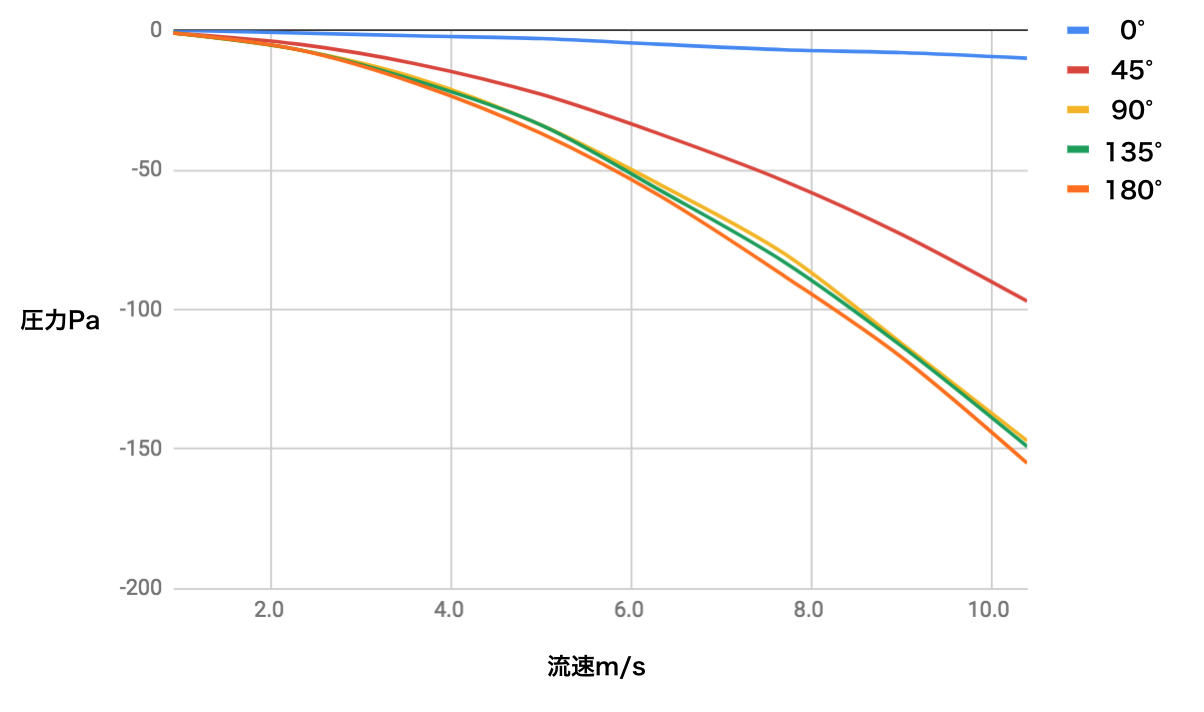
\includegraphics[width=7cm]{../img/graph1.png}
        \caption{定点での圧力測定結果}
      \end{center}
    \end{figure}

  \subsection{円柱周りの圧力分布の測定}
    % 円柱周りの圧力分布の測定
    結果を表5,6,7に示した.また,円柱周りの圧力測定結果を図16,17,18に示した.なお,
    ポテンシャル理論に基づく円柱表面の圧力分布の理論式(7)から得られた結果も示した.
    \begin{eqnarray}
      P = \frac{1}{2} \rho U_{R}^2(1-4 \sin^2 \theta)
    \end{eqnarray}
      % 表5
      \begin{table}[]
        \centering
          \caption{$E_{v}=0.04$Vのときの円柱周りの圧力測定結果}
          \label{my-label}
          \footnotesize
          \begin{tabular}{llll}
            $角度^\circ$ & 圧力 $P_{M}$ Pa & 修正圧力 $P_{R}$ Pa & 理論圧力Pa Pa\\ \hline
            0	& -4 & 	11&  	15 \\
            15&	-6 & 	9 & 	11  \\
            30&-12&3&0  \\
            45&-23& 	-8& 	-15  \\
            60&	-33& 	-18& 	-30  \\
            75&	-36& 	-21& 	-41  \\
            90&	-33& 	-18& 	-45  \\
            105&-34& 	-19& 	-41  \\
            120	&-33& 	-18& 	-30  \\
            135&	-34& 	-19& 	-15  \\
            150&-34& 	-19& 	0  \\
            165&	-36& 	-21& 	11  \\
            180&	-36& 	-21& 	15  \\
            195&	-36& 	-21& 	11  \\
            210&	-35& 	-20& 	0  \\
            225&	-34& 	-19& 	-15  \\
            240&	-34& 	-19& 	-30  \\
            255&	-33& 	-18& 	-41  \\
            270&	-34& 	-19& 	-45  \\
            285&	-37& 	-22& 	-41  \\
            300&	-34& 	-19& 	-30  \\
            315&	-23& 	-8& 	-15  \\
            330&	-13& 	2& 	0  \\
            345&	-6& 	9& 	11 \\ 
            360&	-3& 		 
          \end{tabular}
      \end{table}

      % 表6
      \begin{table}[]
        \centering
          \caption{$E_{v}=0.06$Vのときの円柱周りの圧力測定結果}
          \label{my-label}
          \footnotesize
          \begin{tabular}{llll}
            $角度^\circ$ & 圧力 $P_{M}$ Pa & 修正圧力 $P_{R}$ Pa & 理論圧力Pa Pa\\ \hline
            0&	-6& 	30& 	36  \\
            15&	-11& 	25& 	26  \\
            30&	-29&	7& 	0  \\
            45&	-54& 	-18& 	-36 \\ 
            60&	-77& 	-41& 	-71  \\
            75&	-86& 	-50& 	-98  \\
            90&	-80& 	-44& 	-107  \\
            105&	-79& 	-43& 	-98  \\
            120&	-80& 	-44& 	-71  \\
            135&	-84& 	-48& 	-36  \\
            150&	-83& 	-47& 	0  \\
            165&	-85& 	-49& 	26  \\
            180&	-89& 	-53& 	36  \\
            195&	-86& 	-50& 	26  \\
            210&	-83& 	-47& 	0  \\
            225&	-82& 	-46& 	-36  \\
            240&	-81& 	-45& 	-71  \\
            255&	-80& 	-44& 	-98  \\
            270&	-80& 	-44& 	-107  \\
            285&	-90& 	-54& 	-98  \\
            300&	-80& 	-44& 	-71  \\
            315&	-56& 	-20& 	-36  \\
            330&	-30& 	6& 	0  \\
            345&	-13& 	23& 	26  \\
            360&	-6& 		 \\
          \end{tabular}
      \end{table}

      % 表7
      \begin{table}[]
        \centering
          \caption{$E_{v}=0.08$Vのときの円柱周りの圧力測定結果}
          \label{my-label}
          \footnotesize
          \begin{tabular}{llll}
            $角度^\circ$ & 圧力 $P_{M}$ Pa & 修正圧力 $P_{R}$ Pa & 理論圧力Pa Pa\\ \hline
            0&	-9&	56 	65  \\
            15&	-18&	47& 	48 \\ 
            30&	-50&	15&	0  \\
            45&	-99&	-34& 	-65 \\ 
            60&	-141&	-76& 	-130  \\
            75&	-158&	-93& 	-178  \\
            90&	-147&	-82& 	-195  \\
            105&	-147&	-82& 	-178  \\
            120&	-145&	-80& 	-130  \\
            135&	-150&	-85& 	-65  \\
            150&	-152&	-87& 	0  \\
            165&	-154&	-89& 	48  \\
            180&	-162&	-97& 	65  \\
            195&	-150&	-85& 	48  \\
            210&	-151&	-86& 	0  \\
            225&	-149&	-84& 	-65  \\
            240&	-150&	-85& 	-130  \\
            255&	-152&	-87&	-178  \\
            270&	-149&	-84& 	-195  \\
            285&	-169&	-104& 	-178  \\
            300&	-148&	-83& 	-130  \\
            315&	-101&	-36& 	-65  \\
            330&	-55&	10& 	0  \\
            345&	-23&	42& 	48  \\
            360&	-10&		
          \end{tabular}
      \end{table}

    \subsection{流れの可視化}
      % TODO: 図を2,3,4,5はる
      結果を図2,3,4,5に示した.それぞれの供試模型における考察を行う.
      \begin{enumerate}
        \item 円柱 \\
          電圧が上昇するにつれて,剥離している部分の輪郭線ははっきり現れている.
          $\theta = 90^\circ, 270^\circ$付近で剥離しており,下流方向に対して
          煙が拡散している.よどみ点で物体と流体が
          衝突するときに運動量が流体から物体へと移るので,流速が上がるにつれ,
          流体の持つ移りきらなかった運動量が大きくなり,煙が広がっていると考えられた.
        \item 正4角形 \\
          迎え角で剥離していた.$theta=40^\circ$の時が煙が一番広がっており,この時が一番
          運動量が物体に移動していたことがわかる.
        \item 翼 \\
          迎え角が小さい場合は剥離は生じてない,つまり抵抗は小さいが,大きい場合は剥離が生じた.
          これは,飛行機のブレーキと同じ仕組みだと思われる.
        \item 自動車 \\
          流速が上がっても剥離点は変わらなかった.しかし,フロントの窓ガラス部に流体がぶつかり,
          下向きの揚力が発生していたと思われる.
      \end{enumerate}

      \begin{figure}[htbp]
        % 図2
        \begin{minipage}{0.5\hsize}
          \begin{center}
            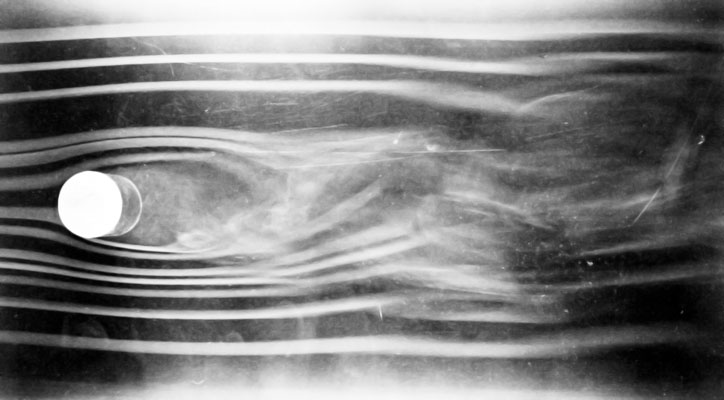
\includegraphics[width=7cm]{../img/kashika/001.jpg}
            \caption{円柱 $E_{R}=0.016V$}
          \end{center}
        \end{minipage}
        \begin{minipage}{0.5\hsize}
          % 図3
          \begin{center}
            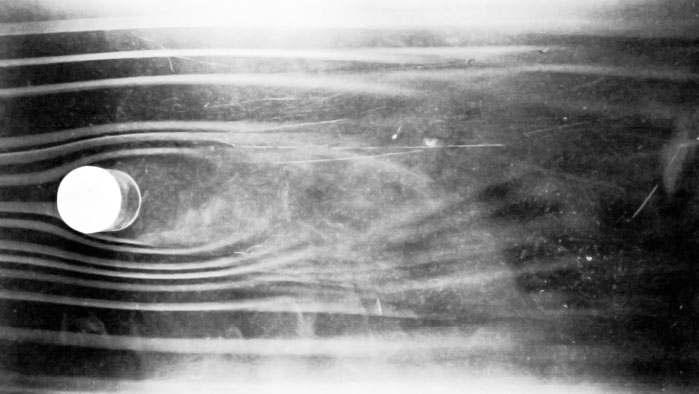
\includegraphics[width=7cm]{../img/kashika/002.jpg}
            \caption{円柱 $E_{R}=0.024V$}
          \end{center}
        \end{minipage}
        \begin{minipage}{0.5\hsize}
          % 図4
          \begin{center}
            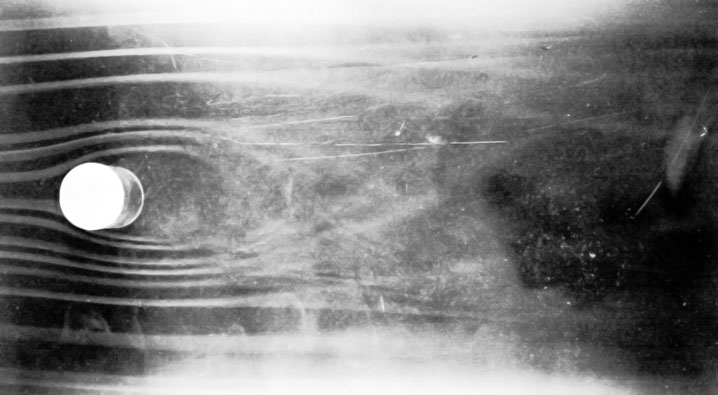
\includegraphics[width=7cm]{../img/kashika/003.jpg}
            \caption{正4角形 $E_{R}=0.016V, \theta=0^\circ$ }
          \end{center}
        \end{minipage}
      \end{figure}

      % 正4角形
      \begin{figure}[htbp]
        % 図5
        \begin{minipage}{0.5\hsize}
          \begin{center}
            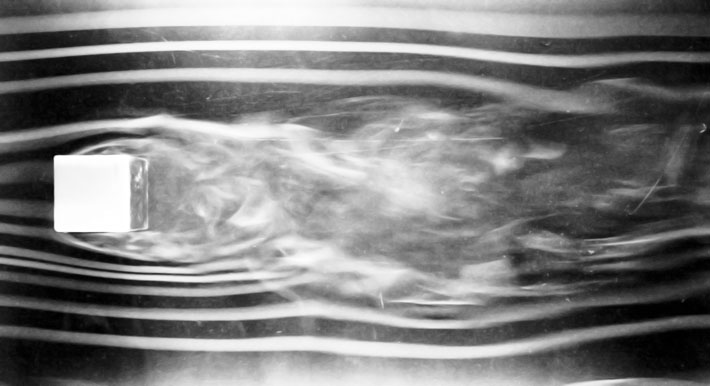
\includegraphics[width=7cm]{../img/kashika/004.jpg}
            \caption{正4角形 $E_{R}=0.016V, \theta=0^\circ$}
          \end{center}
        \end{minipage}
        \begin{minipage}{0.5\hsize}
          % 図6
          \begin{center}
            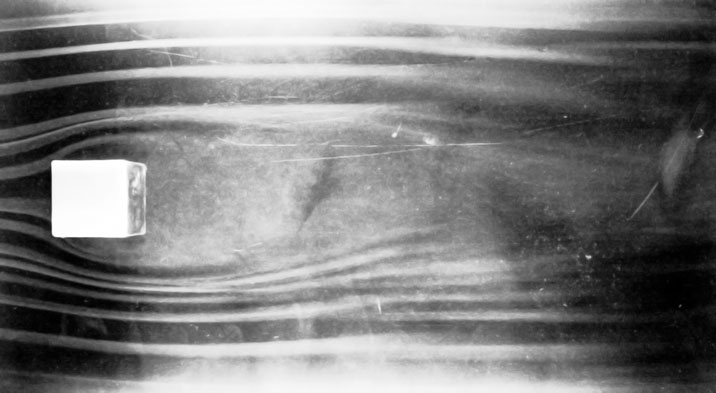
\includegraphics[width=7cm]{../img/kashika/005.jpg}
            \caption{正4角形 $E_{R}=0.025V, \theta=0^\circ$}
          \end{center}
        \end{minipage}
        \begin{minipage}{0.5\hsize}
          % 図7
          \begin{center}
            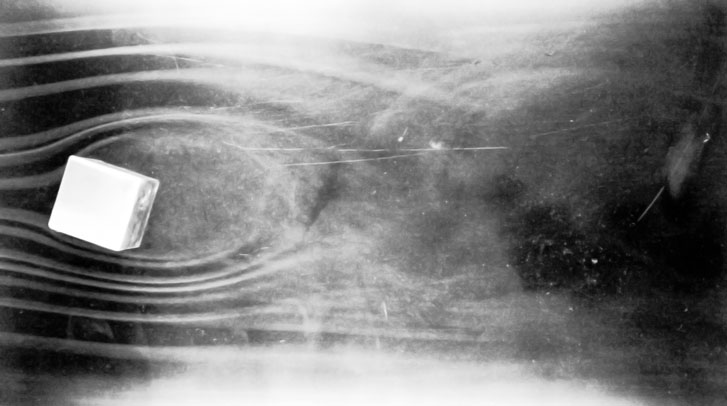
\includegraphics[width=7cm]{../img/kashika/006.jpg}
            \caption{正4角形 $E_{R}=0.025V, \theta=20^\circ$}
          \end{center}
        \end{minipage}
        \begin{minipage}{0.5\hsize}
          % 図8
          \begin{center}
            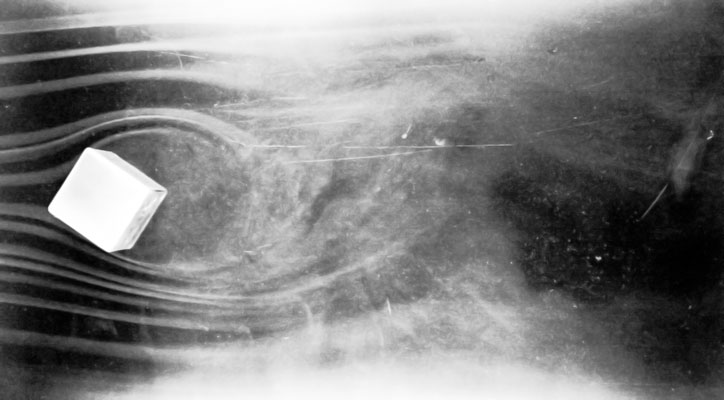
\includegraphics[width=7cm]{../img/kashika/007.jpg}
            \caption{正4角形 $E_{R}=0.025V, \theta=40^\circ$}
          \end{center}
        \end{minipage}
      \end{figure}

      % 翼
      \begin{figure}[htbp]
        % 図8
        \begin{minipage}{0.5\hsize}
          \begin{center}
            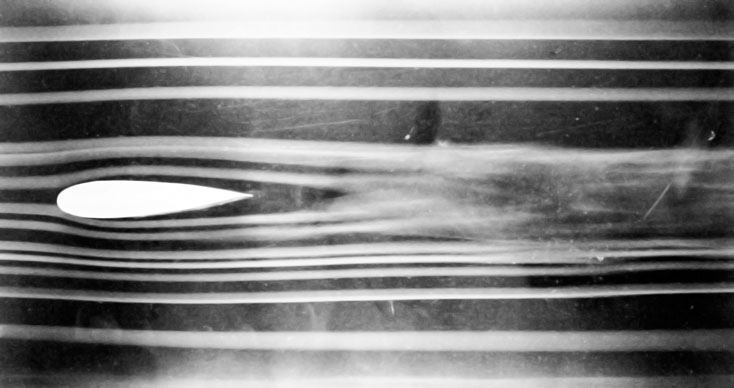
\includegraphics[width=7cm]{../img/kashika/008.jpg}
            \caption{正4角形 $E_{R}=0.022V, \theta=0^\circ$}
          \end{center}
        \end{minipage}
        \begin{minipage}{0.5\hsize}
          % 図9
          \begin{center}
            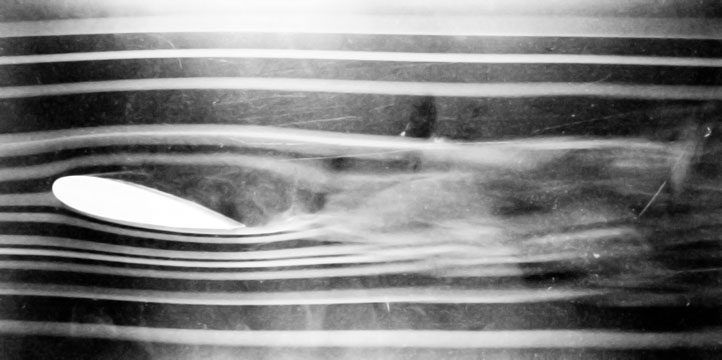
\includegraphics[width=7cm]{../img/kashika/009.jpg}
            \caption{正4角形 $E_{R}=0.022V, \theta=-20^\circ$}
          \end{center}
        \end{minipage}
        \begin{minipage}{0.5\hsize}
          % 図10
          \begin{center}
            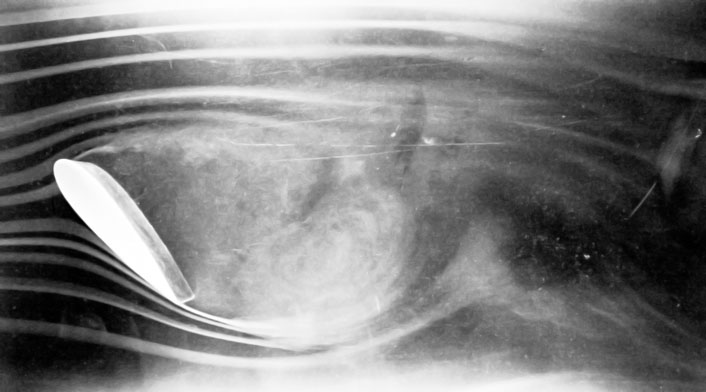
\includegraphics[width=7cm]{../img/kashika/010.jpg}
            \caption{正4角形 $E_{R}=0.026V, \theta=-70^\circ$}
          \end{center}
        \end{minipage}
        \begin{minipage}{0.5\hsize}
          % 図11
          \begin{center}
            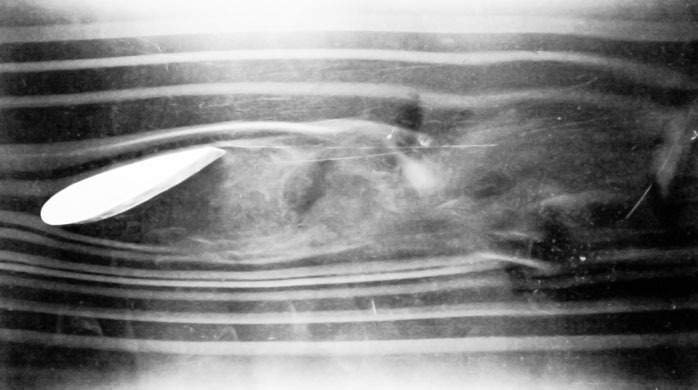
\includegraphics[width=7cm]{../img/kashika/011.jpg}
            \caption{正4角形 $E_{R}=0.026V, \theta=20^\circ$}
          \end{center}
        \end{minipage}
      \end{figure}

      % 自動車
      \begin{figure}[htbp]
        % 図12
        \begin{minipage}{0.5\hsize}
          \begin{center}
            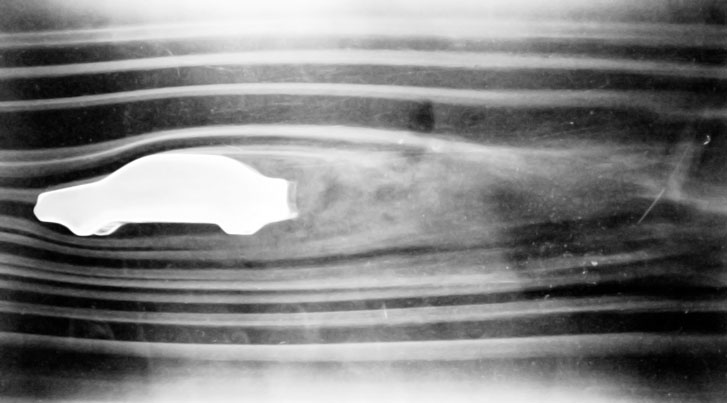
\includegraphics[width=7cm]{../img/kashika/012.jpg}
            \caption{自動車 $E_{R}=0.022V$}
          \end{center}
        \end{minipage}
        \begin{minipage}{0.5\hsize}
          % 図13
          \begin{center}
            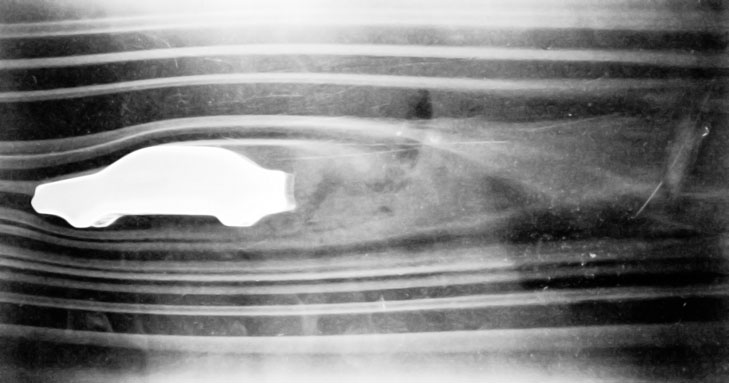
\includegraphics[width=7cm]{../img/kashika/013.jpg}
            \caption{自動車 $E_{R}=0.025V$}
          \end{center}
        \end{minipage}
        \begin{minipage}{0.5\hsize}
          % 図14
          \begin{center}
            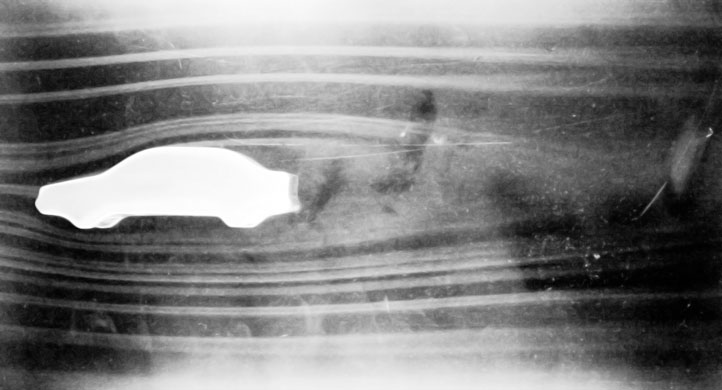
\includegraphics[width=7cm]{../img/kashika/014.jpg}
            \caption{自動車 $E_{R}=0.036V$}
          \end{center}
        \end{minipage}
      \end{figure}


\section{課題}
  \subsection{淀み点の圧力}
    本実験装置で円柱をおいた場合にベルヌーイの式を適用すると,(8)が成り立つ.
    $v_{A}$は風洞外の流速,$P_{A}$は大気圧,$v_{W}$は吸い込み式風洞内の流速,
    $P_{W}$は吸い込み式風洞内の圧力である.
    \par 吸い込み式風洞の場合,点Aは風洞の外を基準としているため$P_{A}$は大気圧と
    等しくなり,$P_{A}$ = $P_{0}$となる.また,流速$v_{A}$も風洞の外の流速を
    基準とするので$v_{A}=0$となり,$P_{W}$は(8)で表せれる.風洞内部の圧力は大気圧よりも低いので
    常に負圧状態であることがわかる.
    \begin{eqnarray}
      % 7,8
      \frac{\rho v_{A}^2}{2} + P_{A} &=& \frac{\rho v_{W}^2}{2} + P_{W} \\
      P_{W} &=&P_{0} -  \frac{\rho v_{W}^2}{2}
    \end{eqnarray}
    \par 次に,吸い込み式風洞外部の点Aと吸い込み式風洞内部に置かれた円筒の淀み点S
    の間でベルヌーイの式を用いると,(10)が成り立つ.また,$p_{A} = p_{0}$,$v_{A}=0$であるので,
    (11)が成り立つ.つまり,風洞内の淀み点圧は大気圧に等しいことがわかる.
    \begin{eqnarray}
      % 9,10
      \frac{\rho v_{A}^2}{2} + P_{A} &=& \frac{\rho v_{S}^2}{2} + P_{S} \\
      P_{S} &=&P_{A}
    \end{eqnarray}
  \subsection{レイノルズ数について}
    (1)の両辺を$\rho$で割ると(12)が得られ,無次元数を用いて方程式系を無次元に書きあらためると,
    方程式は(13)となる.よって,レイノルズ数を用いて表すと(14)となり,パラメータはレイノルズ数
    のみであることがわかる.無次元数は,\\
    $t' = \frac{t}{\frac{L}{U}}, x'=\frac{x}{L}, y'=\frac{y}{L}, u'=\frac{u}{U}, v'=\frac{v}{U}, p'=\frac{p}{\rho U^2}$
    である.
      \begin{eqnarray}
        % 11, 12, 13
        \left( \frac{\partial u}{\partial t} + u\frac{\partial u}{\partial x} + v\frac{\partial u}{\partial y} \right) &=& - \frac{\partial \frac{p}{\rho}}{\partial x} + \frac{\mu}{\rho} \left( \frac{\partial^2 u}{\partial x^2} + \frac{\partial^2 u}{\partial y^2} \right) \nonumber \\
        \\
        P_{S} &=&P_{A} \\
        \left( \frac{\partial u'}{\partial t'} + u'\frac{\partial u'}{\partial x'} + v'\frac{\partial u'}{\partial y'} \right) &=& - \frac{\partial p'}{\partial x'} + \frac{1}{Re} \left( \frac{\partial^2 u'}{\partial x'^2} + \frac{\partial^2 u'}{\partial y'^2} \right) \nonumber \\
      \end{eqnarray}
  \subsection{現象を無次元化してかんが得ることの流体力学的意味と重要性}
    流体力学の研究においては実寸大での実験を行う
    ことは困難なため,相似な模型を用いて実験を行うことが多い.そのときに,無次元量を
    扱うことで実寸大であろうが,模型だろうが関係なく(14)を適用できるので,楽である.
    また,実験での
    流体が実際の流体と本質的に同じになる必要がある.無次元の
    値を用いることで,この関係を導くことが容易になるので,無次元を使うことが
    重要である.
  \subsection{スモークワイヤ法の原理と可視化した現象}
    スモークワイヤー法とは,気体流れ中に張られた金属細線に,トレーサーと呼ばれる油を塗
    布し,細線に電圧をかけ発熱させることで煙を発生させ,この煙を利用して流れの可視化を行
    う方法である.[2]
\section{感想}
  \subsection{実験時の役割について}
    電圧を読み取った.電圧を読み取ると同時に,角度$\theta$もみていため,直感的に実験がわかりやすかった.
  \subsection{実験の感想および批判}
    身の周りの不思議に思っていたことが,次々に流体現象で説明できることがわかり,感動した.
    今までの実験の中で一番楽しかった.
  \subsection{レポート作成に当たって工夫したこと}
    当時の光景を思い返しながら執筆した.また,配られたレポートの書き方手順書全てに従うことはせずに,
    少し変えながらやってしまった.

\begin{thebibliography}{3}
  \bibitem{}知能機械工学基礎実験テキスト P.111-P.124
  \bibitem{}池田 悠太,33 スモークワイヤー法による流れの可視化,http://www.nagaoka-ct.ac.jp/me/events/presen/H16-33.pdf

\end{thebibliography}
\end{document}